\documentclass{beamer}
\usetheme{Madrid} % My favorite!
%\usecolortheme{seahorse} % Simple and clean template
%\usetheme{Darmstadt} % not so good
% Uncomment the following line if you want %
% page numbers and using Warsaw theme%
 \setbeamertemplate{footline}[page number]
\setbeamercovered{transparent}
%\setbeamercovered{invisible}
% To remove the navigation symbols from 
% the bottom of slides%
\setbeamertemplate{navigation symbols}{} 
%
\usepackage{graphicx}
%\usepackage{bm}         % For typesetting bold math (not \mathbold)
\logo{
\includegraphics[height=0.6cm]{di}}
%
\title[The BufferBloar Phenomenon]{Testing, Detection and Possible solutions for the BufferBloat Phenomenon}
\author{Juan S. Catal\'an Olmos}
\institute[UTFSM]
{
Universidad T\'ecnica Federico Santa Mar\'ia\\
\medskip
{\emph{Computer Science Department}}
}
\date{\today}
% \today will show current date. 
% Alternatively, you can specify a date.
%
\begin{document}
%
\begin{frame}
\titlepage
\end{frame}
%
\begin{frame}
\frametitle{Motivation}
\begin{block}{}
\textit{Lets think of a network as a road system where everyone drives at the maximum speed. When the road gets full, there are only two choices: crash into other cars, or get off the road and wait until things get better. The former isn't as disastrous on a network as it would be in real life: losing packets in the middle of a communication session isn't a big deal. But making a packet wait for a short time is usually better than ``dropping" it and having to wait for a retransmission.}[iv]
\end{block}
\end{frame}
%
\begin{frame}
\frametitle{Preliminary Thoughts}
\begin{block}{Study Cases}
\begin{center}
\begin{itemize}
\item Real Time Applications
\item Live Steaming
\item Online Gaming
\end{itemize}
\end{center}
\end{block}
\begin{figure}[htp]
\centering
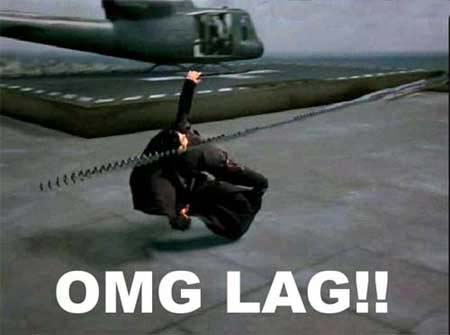
\includegraphics[scale=0.4]{/home/ess/Windows/Documents/Ramos/20112/SEMMEM/git/Presentacion_prelim/omfg-lag.jpg}
\label{lag}
\end{figure}
\end{frame}
%
\begin{frame}
\frametitle{Problem Definition}
\begin{block}{}
Unnecessary latency and poor system performance.
\end{block}
\begin{block}{The Culprit}
Bufferbloat, the existence of excessively large and frequently full buffers inside the network.
\end{block}
\begin{block}{}
 Long delays from bufferbloat are frequently attributed incorrectly to network congestion, and this misinterpretation of the problem leads to the wrong solutions being proposed.
\end{block}
\end{frame}
%
\begin{frame}
\frametitle{Objectives}
\begin{block}{General}
\begin{center}
\begin{itemize}
\item To explain the \textit{BufferBloat} phenomenon, and explain the impact that it could have over the lantecy and throughtput in Internet.
\item To detect the presence by a empirical mesure of the latency and throughput in a TCP/IP based networks.
\item To propose possible solutions in the implementation of a network where the existence of excessively large and frequently full buffers are detected, by mesuring and modeling the effects.
\end{itemize}
\end{center}
\end{block}
\end{frame}
%
\begin{frame}
\frametitle{Objectives}
\begin{block}{Specific}
\begin{center}
\begin{itemize}
\item To select or develop appropriate test to be able to prove the existence of \textit{Bufferbloat}.
\item To test and differentiate the possible cause of the excesive latency and throughput in a TCP/IP LAN and proof how much is generated by the \textit{Bufferbloat} or by a miss-configuration.
\item To propose a possible configuration of the TCP parameters in a Linux based machine or an algorithm that can help to minimize the phenomenon.
\end{itemize}
\end{center}
\end{block}
\end{frame}
%
\begin{frame}
\frametitle{Diagnosing}
\begin{block}{}
BufferBloat's existence is pretty easy to figure out; identifying which hop is the current curlpit is harder.
\end{block}
\begin{block}{Theoretical}
\begin{center}
\begin{itemize}
\item RFC 793,2001,896,879,...
\item ACM - SIGCOMM
\item Others
\end{itemize}
\end{center}
\end{block}
\begin{block}{Experiential}
\begin{center}
\begin{itemize}
\item ICSI Netalyzer
\item Smokeping
\item Wireshark
\end{itemize}
\end{center}
\end{block}
\end{frame}
%
\begin{frame}
\frametitle{Workflow}
\begin{center}\begin{tabular}{|p{9cm}|p{2cm}|}
\hline
Activity & \centerline{Duration}\centerline{(weeks)}\\
\hline
	Definition and understanding of the key concepts related with the \textit{BufferBloat} phenomenon & \centerline{3}\\
\hline
	Research and develop the state of art of the \textit{BufferBloat} phenomenon and the related technologies & \centerline{4} \\
\hline
	To develop and apply different kind of tests to detect the existence of the phenomenon & \centerline{5}\\
\hline
 To mount and test different TCP configurations in a linux machine and OpenWRT router.& \centerline{4}\\
\hline
	Analysis of results and search of possible solutions & \centerline{5}\\
\hline
Final review and corrections & \centerline{3}\\
\hline
TOTAL & \centerline{24}\\
\hline
\end{tabular}\end{center}

\end{frame}
%
\begin{frame}
\frametitle{References}
\begin{enumerate}[i.-]
\item \textit{Bufferbloat: Dark Buffers in the Internet}\\
	Author: Jim Gettys, Kathleen Nichols\\
	Published: Queue vol. 9, no. 11, November 29, 2011\\
\item \textit{BufferBloat: What's Wrong with the Internet?}\\
	Published: Queue vol. 9, no. 12, December 7, 2011\\
\item \textit{jg's Ramblings}\\
	Author: Jim Gettys\\
	\url{http://gettys.wordpress.com/}\\
\item \textit{Understanding bufferbloat and the network buffer arms race}\\
	\url{http://arstechnica.com/tech-policy/news/2011/01/}\\
	\url{understanding-bufferbloat-and-the-network-buffer-arms-race.ars}\\
\item \textit{BufferBloat}\\
	\url{http://www.bufferbloat.net/}\\
\end{enumerate}
\end{frame}
%
\begin{frame}
\centerline{The End (?)}
\vfill
\centerline{\footnotesize{Questions $->$ \url{www.google.com}}}
\end{frame}
% End of slides
\end{document} 
